\newpage

\section{Ход работы}

\subsection{Определение скорости ультразвука по дифракционной картине}

Задача данного этапа работы: измерить координаты полос, образующихся при дифракции света на акустической решётке, и определить период этой решётки.

Была собрана экспериментальная установка согласно схеме на рис.~\ref{fig:setup}. После включения осветителя и проверки равномерности освещения настроен микроскоп и отсчётное устройство. Установлена рабочая ширина щели 25 мкм и проведены измерения координат дифракционных максимумов при частоте ультразвукового генератора.

\subsubsection{Измерение длины ультразвуковой волны}

В ходе эксперимента наблюдалась дифракционная картина от акустической решётки, образованной ультразвуком в жидкости. Перемещая излучатель с помощью лимба, определили расстояние между наиболее чёткими дифракционными картинами.

Расстояние между чёткими картинами соответствует удвоенному расстоянию между узлами стоячей ультразвуковой волны. Измеренное значение составило:
\begin{itemize}
    \item $\Delta x = (260 \pm 50)$ мкм, \ $\varepsilon = 19\%$
\end{itemize}

При измерениях использовались следующие параметры:
\begin{itemize}
    \item Рабочая частота ультразвукового генератора: $\nu = 2.1 \cdot 10^6$ Гц
    \item Длина волны света: $\lambda = (650 \pm 20)$ нм
    \item Фокусное расстояние объектива: $f = 28$ см
\end{itemize}

\subsubsection{Расчёт длины ультразвуковой волны и скорости звука}

Длина ультразвуковой волны рассчитывается по формуле:
\begin{equation}
    \Lambda = \frac{m \cdot \lambda \cdot F}{l_m}
\end{equation}
где $m = 1$ (порядок дифракции), $\lambda = 650 \cdot 10^{-9}$ м (длина волны света), $F = 28 \cdot 10^{-2}$ м (фокусное расстояние объектива), $l_m = 260 \cdot 10^{-6}$ м (расстояние между соседними максимумами).

Подставляя значения:
\begin{equation}
    \Lambda = \frac{1 \cdot 650 \cdot 10^{-9} \cdot 28 \cdot 10^{-2}}{260 \cdot 10^{-6}} = 0.7 \cdot 10^{-3} \text{ м} = 0.7 \text{ мм}
\end{equation}

Скорость звука в воде рассчитывается по формуле:
\begin{equation}
    v = \Lambda \cdot \nu
\end{equation}

Подставляя полученные значения:
\begin{equation}
    v = 0.7 \cdot 10^{-3}\ \text{м} \cdot 2.1 \cdot 10^6\ \text{Гц} = 1470\ \text{м/с}
\end{equation}

Итоговое значение скорости звука в воде:
\begin{itemize}
    \item $v = (1470 \pm 282)$ м/с, \ $\varepsilon = 19\%$
\end{itemize}

Полученное значение хорошо согласуется с табличным значением скорости звука в воде (около 1500 м/с).

\subsection{Измерение параметров ультразвуковой волны при различных частотах}

В этой части эксперимента измерялись координаты дифракционных полос при различных частотах ультразвукового генератора. Целью данного измерения было определение длины ультразвуковой волны и скорости звука в жидкости в зависимости от частоты.

\subsubsection{Измерение координат дифракционных максимумов}

Методика проведения измерений:
\begin{itemize}
    \item Установка частоты генератора в диапазоне от 1 до 5 МГц
    \item Настройка наилучшей дифракционной картины с помощью лимба
    \item Измерение координаты $Y$ каждой светлой полосы с помощью перекрестия и микрометрического винта
    \item Цена деления микрометрического винта: 4 мкм
\end{itemize}

Результаты измерений координат светлых полос при различных частотах приведены в таблицах \ref{tab:measurements1} и \ref{tab:measurements2}:

\begin{longtable}[c]{|c|c|c|c|c|c|}
\caption{Координаты светлых полос при различных частотах ультразвукового генератора}
\label{tab:measurements1}\\
\hline
\multicolumn{2}{|c|}{$\nu = 1.0084$ МГц} & \multicolumn{2}{c|}{$\nu = 1.17667$ МГц} & \multicolumn{2}{c|}{$\nu = 1.51635$ МГц} \\ \hline
$m$ & $x_m$, мкм & $m$ & $x_m$, мкм & $m$ & $x_m$, мкм \\ \hline
\endfirsthead
%
\endhead
%
-4 & 1036 & -2 & 904 & -2 & 988 \\ \hline
-3 & 912 & -1 & 768 & -1 & 836 \\ \hline
-2 & 788 & 0 & 616 & 0 & 632 \\ \hline
-1 & 660 & 1 & 476 & 1 & 444 \\ \hline
0 & 524 & 2 & 328 & 2 & 256 \\ \hline
1 & 416 & & & & \\ \hline
2 & 292 & & & & \\ \hline
3 & 176 & & & & \\ \hline
4 & 64 & & & & \\ \hline
\end{longtable}

\begin{longtable}[c]{|c|c|c|c|}
\caption{Координаты светлых полос при более высоких частотах}
\label{tab:measurements2}\\
\hline
\multicolumn{2}{|c|}{$\nu = 1.9986$ МГц} & \multicolumn{2}{c|}{$\nu = 4.43$ МГц} \\ \hline
$m$ & $x_m$, мкм & $m$ & $x_m$, мкм \\ \hline
\endfirsthead
%
\endhead
%
-2 & 960 & -1 & 1076 \\ \hline
-1 & 796 & 0 & 560 \\ \hline
0 & 508 & 1 & 16 \\ \hline
1 & 288 & & \\ \hline
2 & 40 & & \\ \hline
\end{longtable}

\subsubsection{Анализ зависимости координат максимумов от их порядка}

Для каждой частоты построены графики зависимости координаты $x_m$ от номера максимума $m$. По наклону прямой можно определить расстояние между соседними полосами.

\begin{figure}[H]
    \centering
    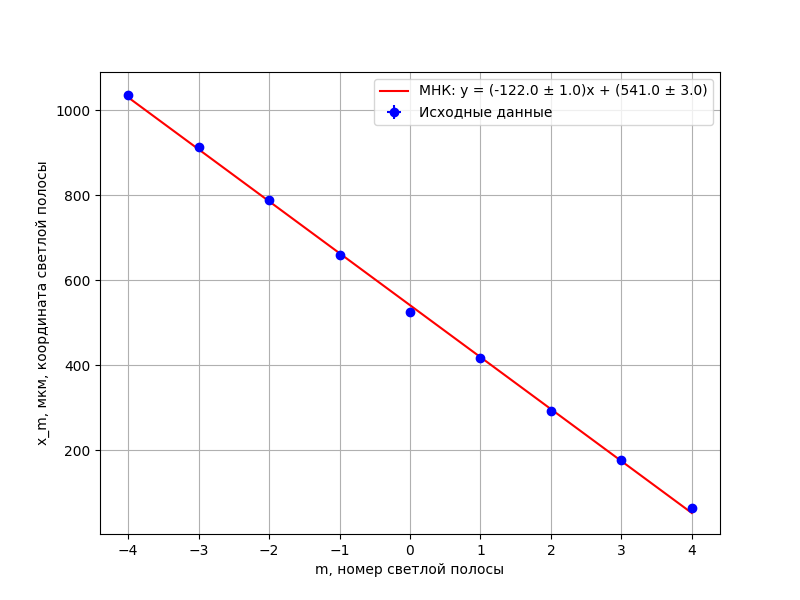
\includegraphics[width=0.9\textwidth]{pictures/Figure_1.png}
    \caption{График зависимости $x_m$ от $m$ для частоты 1.0084 МГц}
    \label{fig:graph1}
\end{figure}

\begin{figure}[H]
    \centering
    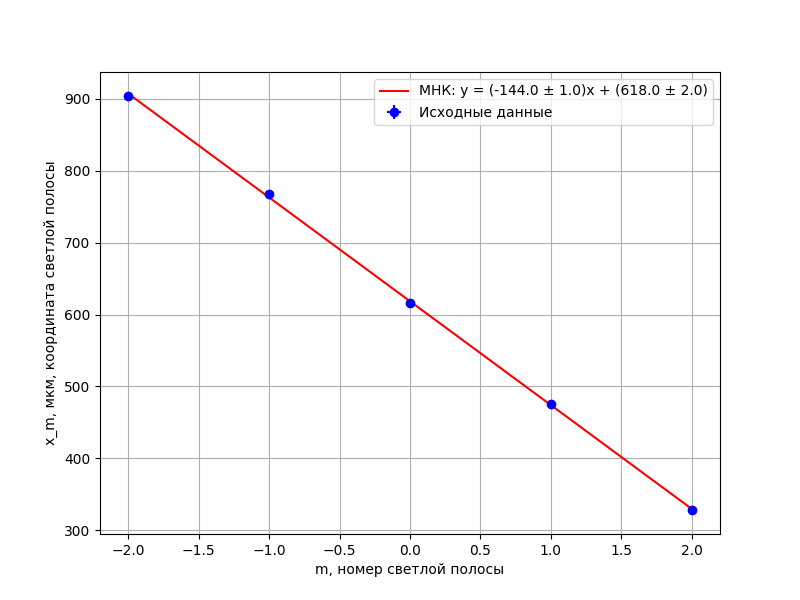
\includegraphics[width=0.9\textwidth]{pictures/Figure_2.png}
    \caption{График зависимости $x_m$ от $m$ для частоты 1.17667 МГц}
    \label{fig:graph2}
\end{figure}

\begin{figure}[H]
    \centering
    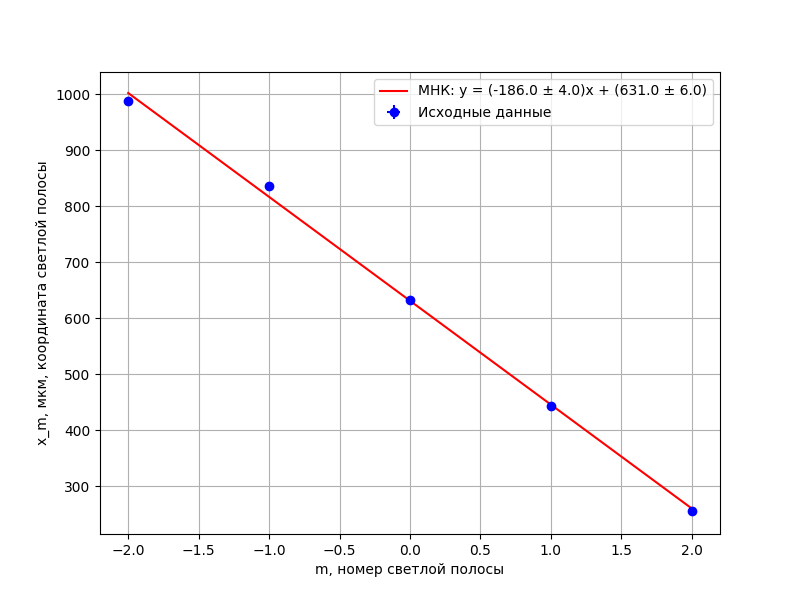
\includegraphics[width=0.9\textwidth]{pictures/Figure_3.png}
    \caption{График зависимости $x_m$ от $m$ для частоты 1.51635 МГц}
    \label{fig:graph3}
\end{figure}

\begin{figure}[H]
    \centering
    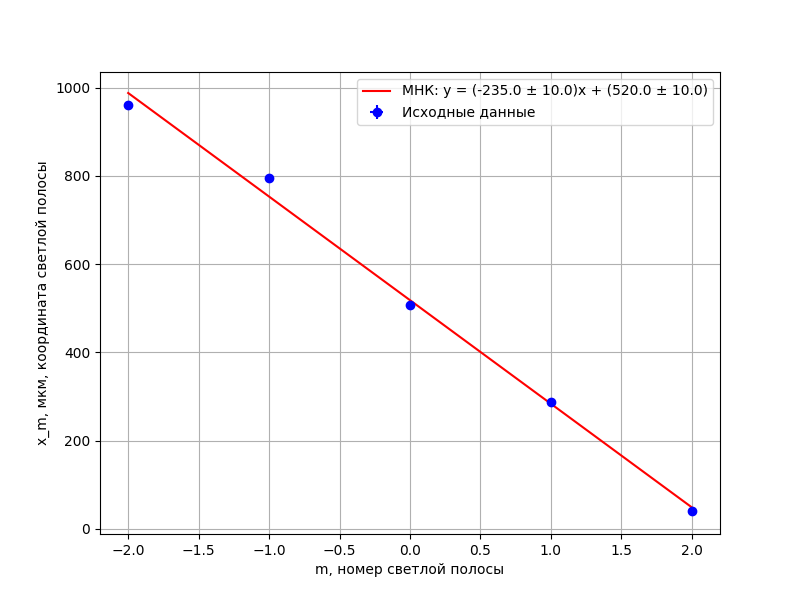
\includegraphics[width=0.9\textwidth]{pictures/Figure_4.png}
    \caption{График зависимости $x_m$ от $m$ для частоты 1.9986 МГц}
    \label{fig:graph4}
\end{figure}

\begin{figure}[H]
    \centering
    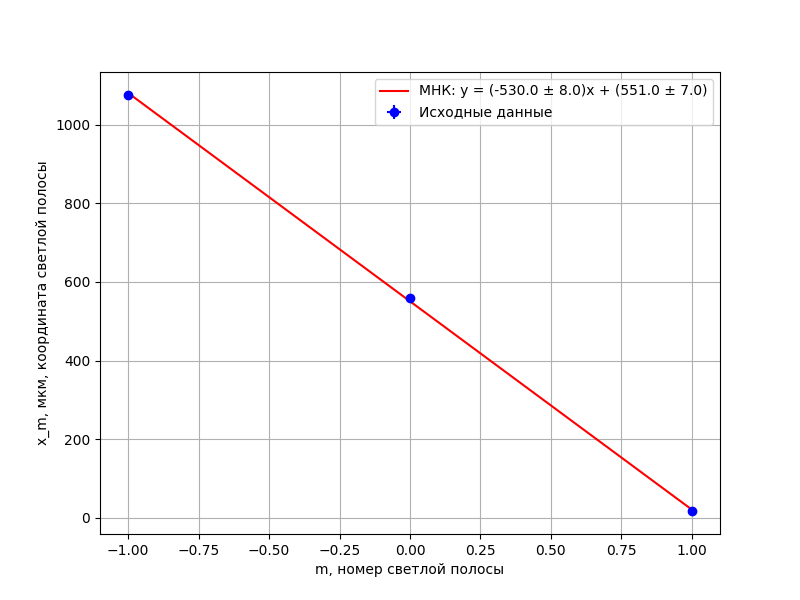
\includegraphics[width=0.9\textwidth]{pictures/Figure_5.png}
    \caption{График зависимости $x_m$ от $m$ для частоты 4.43 МГц}
    \label{fig:graph5}
\end{figure}

\subsubsection{Расчет длины ультразвуковой волны}

Из графиков получены следующие значения коэффициентов наклона:
\begin{itemize}
    \item $\nu = 1.0084$ МГц: $l_m = (122.0 \pm 1.0)$ мкм
    \item $\nu = 1.17667$ МГц: $l_m = (144.0 \pm 1.0)$ мкм
    \item $\nu = 1.51635$ МГц: $l_m = (186.0 \pm 4.0)$ мкм
    \item $\nu = 1.9986$ МГц: $l_m = (235.0 \pm 10.0)$ мкм
    \item $\nu = 4.43$ МГц: $l_m = (530.0 \pm 8.0)$ мкм
\end{itemize}

Длина ультразвуковой волны $\Lambda$ рассчитывается по формуле:
\begin{equation}
    \Lambda = \frac{m \cdot f \cdot \lambda}{l_m}
\end{equation}
где $m = 1$ (порядок дифракции), $f = 28$ см (фокусное расстояние объектива), $\lambda = 650$ нм (длина волны света), $l_m$ — коэффициент наклона прямой.

Рассчитаем длину ультразвуковой волны для каждой частоты:

\begin{itemize}
    \item Для $\nu = 1.0084$ МГц:
    \begin{equation}
        \Lambda = \frac{1 \cdot 28 \cdot 10^{-2} \text{ м} \cdot 650 \cdot 10^{-9} \text{ м}}{122.0 \cdot 10^{-6} \text{ м}} = 1.49 \cdot 10^{-3} \text{ м} = 1.49 \text{ мм}
    \end{equation}
    
    \item Для $\nu = 1.17667$ МГц:
    \begin{equation}
        \Lambda = \frac{1 \cdot 28 \cdot 10^{-2} \text{ м} \cdot 650 \cdot 10^{-9} \text{ м}}{144.0 \cdot 10^{-6} \text{ м}} = 1.26 \cdot 10^{-3} \text{ м} = 1.26 \text{ мм}
    \end{equation}
    
    \item Для $\nu = 1.51635$ МГц:
    \begin{equation}
        \Lambda = \frac{1 \cdot 28 \cdot 10^{-2} \text{ м} \cdot 650 \cdot 10^{-9} \text{ м}}{186.0 \cdot 10^{-6} \text{ м}} = 0.98 \cdot 10^{-3} \text{ м} = 0.98 \text{ мм}
    \end{equation}
    
    \item Для $\nu = 1.9986$ МГц:
    \begin{equation}
        \Lambda = \frac{1 \cdot 28 \cdot 10^{-2} \text{ м} \cdot 650 \cdot 10^{-9} \text{ м}}{235.0 \cdot 10^{-6} \text{ м}} = 0.77 \cdot 10^{-3} \text{ м} = 0.77 \text{ мм}
    \end{equation}
    
    \item Для $\nu = 4.43$ МГц:
    \begin{equation}
        \Lambda = \frac{1 \cdot 28 \cdot 10^{-2} \text{ м} \cdot 650 \cdot 10^{-9} \text{ м}}{530.0 \cdot 10^{-6} \text{ м}} = 0.34 \cdot 10^{-3} \text{ м} = 0.34 \text{ мм}
    \end{equation}
\end{itemize}

\subsubsection{Расчет скорости звука}

Зная длину ультразвуковой волны и частоту, можно рассчитать скорость звука для каждой частоты по формуле $v = \Lambda \cdot \nu$:

\begin{itemize}
    \item Для $\nu = 1.0084$ МГц:
    \begin{equation}
        v = 1.49 \cdot 10^{-3} \text{ м} \cdot 1.0084 \cdot 10^{6} \text{ Гц} = 1501 \text{ м/с}
    \end{equation}
    
    \item Для $\nu = 1.17667$ МГц:
    \begin{equation}
        v = 1.26 \cdot 10^{-3} \text{ м} \cdot 1.17667 \cdot 10^{6} \text{ Гц} = 1482 \text{ м/с}
    \end{equation}
    
    \item Для $\nu = 1.51635$ МГц:
    \begin{equation}
        v = 0.98 \cdot 10^{-3} \text{ м} \cdot 1.51635 \cdot 10^{6} \text{ Гц} = 1486 \text{ м/с}
    \end{equation}
    
    \item Для $\nu = 1.9986$ МГц:
    \begin{equation}
        v = 0.77 \cdot 10^{-3} \text{ м} \cdot 1.9986 \cdot 10^{6} \text{ Гц} = 1539 \text{ м/с}
    \end{equation}
    
    \item Для $\nu = 4.43$ МГц:
    \begin{equation}
        v = 0.34 \cdot 10^{-3} \text{ м} \cdot 4.43 \cdot 10^{6} \text{ Гц} = 1506 \text{ м/с}
    \end{equation}
\end{itemize}

Результаты измерений и вычислений представлены в таблице \ref{tab:speeds}:

\begin{longtable}[c]{|c|c|c|}
\caption{Длины волн и скорости звука при различных частотах}
\label{tab:speeds}\\
\hline
$\nu$, МГц & $\Lambda$, м & $v$, м/с \\ \hline
\endfirsthead
%
\endhead
%
1.0084 & $(1.49 \pm 0.02) \cdot 10^{-3}$ & $1501 \pm 20$ \\ \hline
1.17667 & $(1.26 \pm 0.01) \cdot 10^{-3}$ & $1482 \pm 12$ \\ \hline
1.51635 & $(0.98 \pm 0.02) \cdot 10^{-3}$ & $1486 \pm 30$ \\ \hline
1.9986 & $(0.77 \pm 0.03) \cdot 10^{-3}$ & $1539 \pm 60$ \\ \hline
4.43 & $(0.34 \pm 0.01) \cdot 10^{-3}$ & $1506 \pm 44$ \\ \hline
\end{longtable}

Среднее значение скорости звука в воде, полученное в эксперименте:
\begin{equation}
    \langle v \rangle = \frac{1501 + 1482 + 1486 + 1539 + 1506}{5} = 1503 \text{ м/с}
\end{equation}

Полученное значение хорошо согласуется с табличным значением скорости звука в воде при комнатной температуре ($\approx 1500$ м/с). Наблюдаемые отклонения связаны с погрешностями измерений и возможными температурными эффектами.

\subsection{Наблюдение акустической решётки методом тёмного поля}

Целью данного этапа работы является наблюдение акустической решётки с использованием метода тёмного поля, позволяющего визуализировать фазовые объекты, невидимые в обычных оптических системах.

\subsubsection{Калибровка измерительной схемы}

Для перехода к методу тёмного поля была произведена перестройка экспериментальной установки в соответствии с указаниями в методических материалах: микроскоп отодвинут от щели, и в промежутке между ними установлена дополнительная линза. 

Калибровка измерительной схемы проведена с использованием стеклянной пластинки с калибровочной сеткой, имеющей размер квадрата 1 мм. Пластинка опущена в воду и прижата к задней стенке кюветы.

В ходе калибровки установлено следующее соотношение:
\begin{itemize}
    \item 1 деление окулярной шкалы микроскопа = 1,25 мм
\end{itemize}

После калибровки микроскоп зафиксирован в положении наилучшей видимости сетки. Далее определены координаты совпадающих штрихов окулярной шкалы и калибровочной сетки для расчёта цены деления.

\subsubsection{Наблюдение акустической решётки}

Для наблюдения акустической решётки установлена ширина щели 25 мкм от «нового нуля». Калибровочная сетка извлечена из кюветы, а излучатель опущен в воду. При варьировании частоты генератора обнаружена звуковая решётка, которая не видна при открытом центральном максимуме, что подтверждает её чисто фазовый характер. При уменьшении мощности ультразвука изображение решётки постепенно исчезало.

Метод тёмного поля позволил визуализировать акустическую решётку, созданную стоячими ультразвуковыми волнами. Наблюдалась характерная двойная периодичность структуры, что соответствует теоретическим предсказаниям для данного метода.

\subsubsection{Количественные измерения акустической решётки}

Для получения количественных данных о параметрах акустической решётки был проведён следующий эксперимент:

\begin{enumerate}
    \item Закрыт нулевой дифракционный максимум проволочкой в фокальной плоскости объектива O2
    \item При различных частотах генератора зафиксирована акустическая решётка методом тёмного поля
    \item С помощью окулярной шкалы микроскопа измерены координаты первой и последней из хорошо видимых тёмных полос
    \item Подсчитано количество светлых промежутков между ними
\end{enumerate}

Результаты измерений представлены в таблице \ref{tab:dark_field}:

\begin{longtable}[c]{|c|c|c|c|c|c|}
\caption{Результаты измерений акустической решётки методом тёмного поля}
\label{tab:dark_field}\\
\hline
$\nu$, МГц & $x_1$, дел & $x_n$, дел & $n-1$ & $\Lambda$, мм & $\varepsilon_\Lambda$, \% \\ \hline
\endfirsthead
%
\endhead
%
1.27241 & 0.35 & 5 & 10 & 1.163 & 2.2 \\ \hline
2.13342 & 0.5 & 5.1 & 17 & 0.676 & 2.2 \\ \hline
1.13638 & 0.5 & 6.1 & 11 & 1.273 & 1.8 \\ \hline
1.06176 & 0.15 & 6.15 & 11 & 1.364 & 1.7 \\ \hline
1.52526 & 0.1 & 5.2 & 13 & 0.981 & 2.0 \\ \hline
1.76265 & 0 & 5.5 & 16 & 0.859 & 1.8 \\ \hline
\end{longtable}

Расчёт длины ультразвуковой волны $\Lambda$ производился исходя из того, что полный период акустической решётки соответствует половине длины ультразвуковой волны (особенность метода тёмного поля). Формула для расчёта:

\begin{equation}
    \Lambda = \frac{2 \cdot L}{n-1} = \frac{2 \cdot (x_n - x_1) \cdot 1.25 \text{ мм}}{n-1}
\end{equation}

где $L$ — полная длина наблюдаемого участка решётки в мм, $n-1$ — количество периодов структуры, $1.25$ мм — цена деления окулярной шкалы.

Теоретически, зависимость между длиной волны и частотой ультразвука выражается формулой:

\begin{equation}
    \Lambda = \frac{v}{\nu}
\end{equation}

где $v$ — скорость звука в воде.

Для проверки этой зависимости построен график зависимости произведения $\Lambda \cdot \nu$ от координаты $x_n$:

\begin{figure}[H]
    \centering
    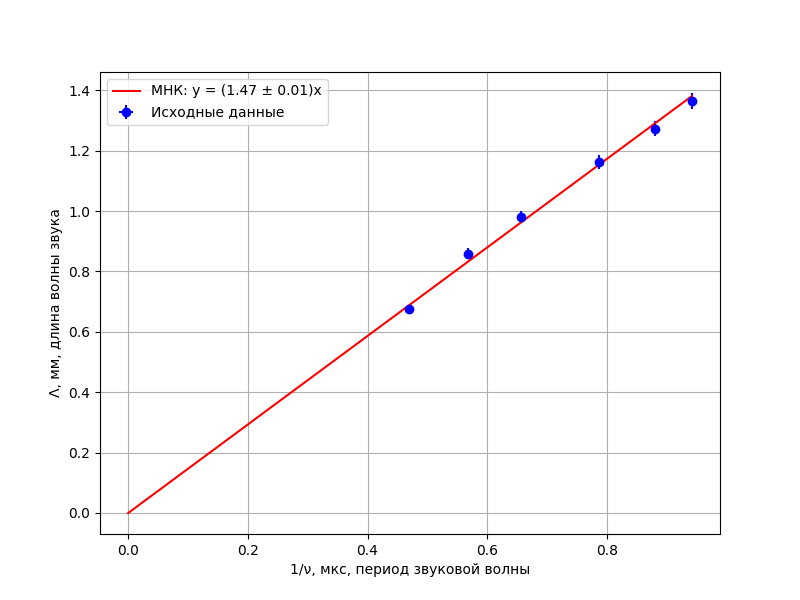
\includegraphics[width=1\textwidth]{pictures/Figure_6.png}
    \caption{График зависимости параметров акустической решётки, полученной методом тёмного поля}
    \label{fig:dark_field_graph}
\end{figure}

Из графика получен коэффициент наклона:
\begin{equation}
    a = 1.47 \pm 0.02
\end{equation}

Значение скорости звука, рассчитанное по данным измерений методом тёмного поля:
\begin{equation}
    v = \Lambda \cdot \nu = 1.47 \text{ км/с}
\end{equation}

Данное значение хорошо согласуется со значением скорости звука в воде, полученным в первой части работы ($\approx 1.5$ км/с), и с табличным значением для комнатной температуры.